\documentclass[11pt,a4paper,spanish]{book}
\usepackage{biblatex}
\usepackage[utf8]{inputenc}
% Imagenes
\usepackage{graphicx, wrapfig, hyperref}
\graphicspath{ {./.images/} }
\usepackage{float}
\usepackage{comment}
\addbibresource{./bibLib/mycol_arte.bib}



\begin{document}
	\chapter{Planteamiento de la comparativa}
	
	En este capítulo se identificará el problema en concreto a tratar, a la vez que el diseño de los experimentos para acometerlo. Para ello se exponen los datos utilizados así como un análisis en detalle de estos respondiendo a por qué se escogen esos conjuntos. Finalmente las técnicas de procesamiento y el diseño de la red neuronal propuesta que se usan en este trabajo
	
	El objetivo de esta comparativa es contrastar los resultados obtenidos tras aplicar el mismo sistema de reconocimiento de emociones en la voz entrenado con un lenguaje de referencia, con los otros dos lenguajes escogidos. Mediante esta comparativa se pretende responder a la pregunta si es posible reconocer emociones en un idioma que en principio se desconoce.
	
	\section{Conjunto de Datos}
	\label{lb_c4_datos}
	Los datos en un proyecto de inteligencia artificial son clave de cara a la obtención de un resultado coherente en nuestro trabajo. Este estudio pretende analizar si es posible clasificar emociones en la lengua extranjera y para encontrar una respuesta, se seguirá la siguiente estrategia con respecto a los datos.
	
	\paragraph{Idioma de referencia: Inglés} El idioma de referencia será el cuál aprenda nuestra red neuronal, y desde el cual se intenten reconocer emociones en otras lenguas. En este caso se propone el inglés.\\
	
	El conjunto de datos que se usará para el idioma de referencia, será La Base de Datos Audiovisual del Discurso y Canción Emocional RAVDESS (por sus siglas en inglés \emph{Ryerson Audio-Visual Database of Emotional Speech and Song}), el cual contiene 7356 archivos en total, entre los cuales podemos encontrar 3 modalidades: sólo audio (en 16 bit, 48 kHz y en formato wav), audio-video (720p H.264, AAC 48kHz, en formato mp4) y sólo video sin sonido. Esta base de datos contiene 24 actores profesionales vocalizando dos frases en inglés norte americano (\emph{Kids are talking by the door} y \emph{Dogs are sitting by the door}).
	
	Cada uno de estos archivos están nombrados de manera única mediante 7 números a modo de descripción de las características del audio. Éste respeta la siguiente convención:
	\begin{itemize}
		\item Modalidad (01 Audio y vídeo, 02 Sólo vídeo, 03 Sólo audio)
		\item Canal vocal (01 discurso normal, 02 canción)
		\item Emoción que representa
		\item Intensidad Emocional Si es normal o fuerte. La voz neutral no contempla la intensidad fuerte.
		\item Repetición (si es la primera repetición 01, si es la segunda 02)
		\item Actor que ejecuta la acción
	\end{itemize}

	Así por ejemplo, el archivo 03-01-03-01-01-01-01.wav dirá que es un archivo de sólo audio (03), donde se vocaliza una frase de manera hablada (01) y con tono alegre (03). La intensidad es normal (01), corresponde a la primera repetición (01) y el actor que la ejecuta es el n.01.
	
	\begin{figure}[H]
		\centering
		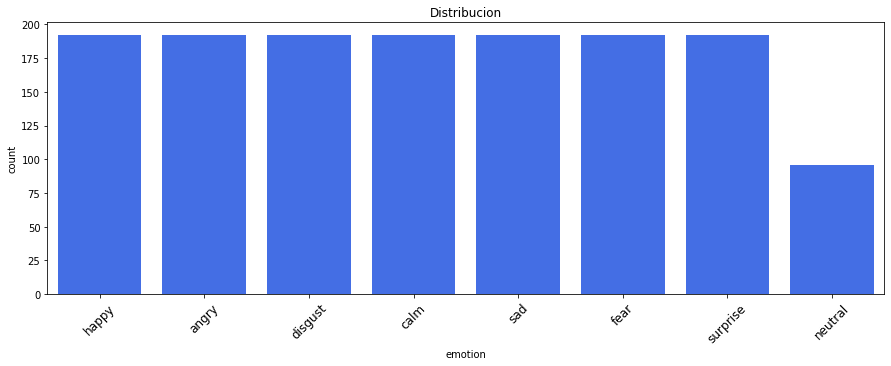
\includegraphics[scale=0.35]{ravdess_distribucion.png} 
		\caption{Distribución de las emociones en RAVDESS}
		\label{fig:emociones_ravdess}
	\end{figure}
	
	Como se puede apreciar en la figura \ref{fig:emociones_ravdess} las emociones están regularmente distribuidas, sin embargo, a pesar de que en este dataset hay 7356 muestras, para este proyecto sólo podremos usar los que presentan una modalidad de sólo audio, lo que nos deja con un total de 1440 muestras. 

	
	\paragraph{Idioma con raíces fonéticas similares: Alemán} Este conjunto de datos pertenecerá a un idioma con unas raíces similares al idioma de referencia, de manera que se espera a priori que se puedan reconocer la mayoría de las emociones.\\
	
	Para este caso el conjunto de datos propuesto es la Base de Datos del Discurso Emocional de Berlín (EMODB, por sus siglas en inglés \emph{Berlin Database of Emotional Speech}). Este corpus contiene 800 grabaciones interpretadas por 10 actores (5 hombres y 5 mujeres) modulando 7 emociones en el idioma alemán. Cada archivo tiene una frecuencia de muestreo de 16 kHz con una resolución de 16 bits, y una duración de 3 segundos de media. Como en el anterior, se utiliza una nomenclatura para nombrar a los archivos que satisface lo siguiente:
	\begin{itemize}
		\item Las dos primeras posiciones determinan el actor que las interpreta.
		\item De la posición 3 a las 5 se define el texto que se pronuncia
		\item La posición 6 indica la emoción.
		\item Versión del audio en caso de que la hubiese (codificado con letras).
	\end{itemize}

	Como ejemplo, el archivo \emph{03a01Fa.wav} indica que el actor 03 (hombre de 31 años) cita el texto a01 (\emph{Der Lappen liegt auf dem Eisschrank}, en alemán "El mantel está colgando del frigo"), con la emoción F (felicidad), y es la versión \emph{a} (la primera).
	
	La documentación del corpus también nos ofrece información sobre el género y edad de los actores, lo cual se ha determinado irrelevante, y las distintas frases que pueden aparecer en los archivos.
	Las emociones que clasifica son enfado (W), aburrimiento (L), asco (E), miedo o ansiedad (A), felicidad (F), tristeza (T) y neutral (N) codificadas en el nombre del archivo por su inicial en alemán (especificada entre paréntesis).


	
	\paragraph{Idioma con raíces fonéticas distintas} Este conjunto de datos pertenecerá a un idioma con unas raíces más distantes al idioma de referencia.\\
	
	
	\section{Extracción de características}
	Teniendo en cuenta el previo estudio de la literatura en el capítulo 2, se concluye que los métodos más prometedores, y que por lo tanto merecen la pena aplicar a este estudio comparativo serían los siguientes:
	\subsubsection{Coeficientes Cepstrales en la escala de Mel}
	Como ya hemos mencionado, MFCC es uno de los mejores algoritmos para capturar características de la señal de audio debido a su similitud a como el sistema auditivo humano procesa el sonido y las frecuencias, así mismo, su efectividad se ha visto reportada y discutida a lo largo de otros estudios.
	La librería usada para la manipulación de audio Librosa ofrece la posibilidad de extraer características MFCC de un archivo de audio. En cuanto a la configuración, se extraerán 13 características MFCC usando el rango de muestreo del propio archivo de audio.

	\begin{comment}
	Razon por el numero de características:
	https://dsp.stackexchange.com/questions/28898/mfcc-significance-of-number-of-features
		Mencionar que otros estudios
	\end{comment}
	
%	\paragraph{Espectogramas de Mel}
%	La escala de Mel transforma  frecuencias lineales a una escala logarítmica

	\section{Configuración}
	En esta sub-sección se muestra los recursos a los que se ha accedido para el desarrollo del estudio, así como su correspondiente configuración.
	\begin{comment}
	\begin{wrapfigure}{l}{0.40\textwidth}
	\vspace{-20pt}
	\centering
	
\includegraphics[width=0.4\linewidth]{/logos/colab_icon.png} 
	\vspace{-20pt}
	\end{wrapfigure}
	\end{comment}
	
	
	\paragraph{Google Colab} Para la exploración de los datos así como el desarrollo, y entrenamiento de los modelos se ha hecho uso de la plataforma gratuita desarrollada por Google, Google Colab. Esta plataforma ofrece 12GB de RAM  y 107.77GB de espacio en disco, que será más que suficiente dado el tamaño que nuestro dataset.
	
	\paragraph{Librosa 0.8.1} Librosa es un paquete que ofrece diversas funcionalidades para el análisis de audio y música, cuya información más en detalle se puede encontrar en \cite{librosa082}. Esta librería ha sido esencial para la extracción de características MFCC así como algunas técnicas de aumento de datos.
	
	\paragraph{Tensorflow 2.0} Es una plataforma de código abierto que provee un conjunto de librerías y recursos para el desarrollo de modelos con aprendizaje automático. Tensorflow, que además ofrece soporte de Keras, se ha usado tanto para la estandarización de los datos, como para la compilación y entrenamiento del modelo.
	
	\paragraph{Python 3} Python es un lenguage interpretado de alto nivel. Todo el código para este proyecto ha sido desarrollado en python 3.
	
	\section{Pre-procesado de los datos}
	Como se ha visto en la sección \ref{lb_c4_datos} no hay una abundante disposición de datos, esto podría convertirse en un problema y perjudicar el rendimiento del modelo en el entrenamiento. 
	Será necesario, antes del entrenamiento, un previo procesado de los datos.
	
	\subsection{División de los datos por género}
	En un primer análisis exploratorio de los datos, se han estudiado las diferencias entre la voz masculina y la voz femenina en las emociones, observando lo siguiente:
	
	\begin{figure}[H]
		\centering
		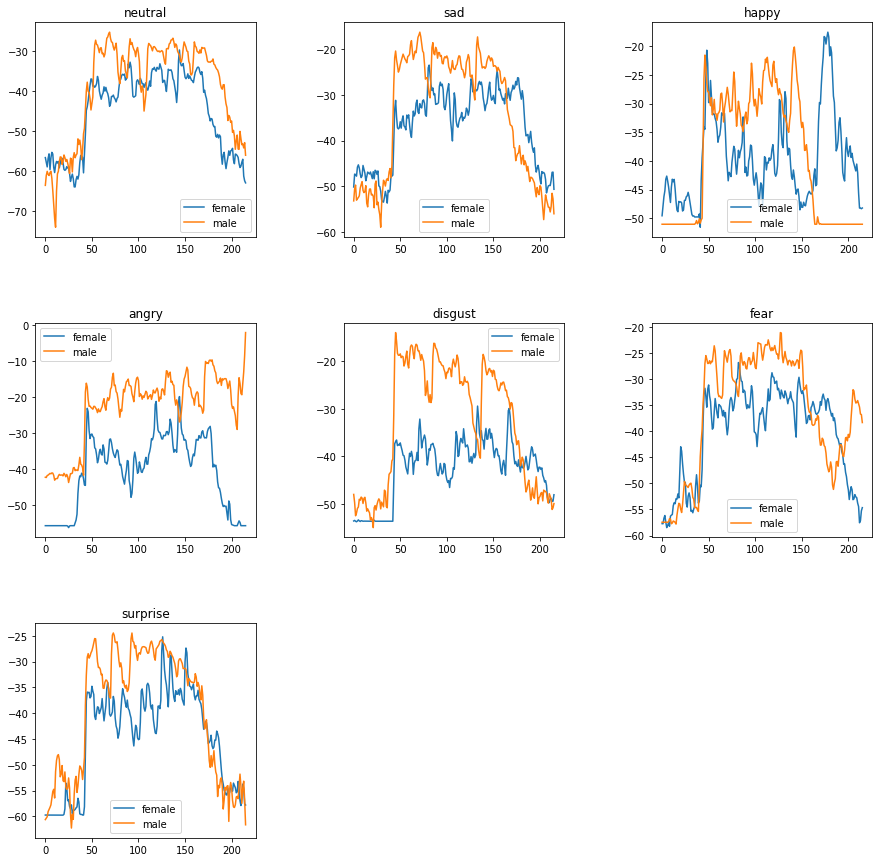
\includegraphics[scale=0.35]{comparative_waveform.png} 
		\caption{Comparativa de los extractos de voz por género en RAVDESS}
		\label{fig:comp_emociones_genero}
	\end{figure}
	En la figura \ref{fig:comp_emociones_genero} podemos ver la comparación de la voz masculina (naranja) y la voz femenina (azul) por cada una de las emociones en el idioma inglés. Ya que es muy distinto, puede ser recomendable dividir el conjunto de datos atendiendo a esta característica.
	
	
	%\subsection{Conversión de la señal a imagen}
	% quiza no sea necesario
	
	%\subsection{Normalización de los datos}
	
	
	\subsection{Ténicas de aumento de datos}
	Dado el bajo número de muestras en los distintos conjuntos de datos a los que hemos podido acceder, se ha visto conveniente explorar distintas técnicas de aumento de datos. El aumento de datos es una técnica por la cual, se aumenta el número de muestras en un conjunto mediante la creación de nuevas muestras sintéticas con pequeñas modificaciones a cada uno de los archivos. Esta aumento de los datos se puede traducir por una reducción del overfitting (sobreajuste), ya que el modelo se mantendría invariable mejorando así su capacidad de generalización.
	Esta técnica es ampliamente conocida cuando se procesan imágenes, siendo esas modificaciones rotaciones, transposiciones etc. En nuestro caso, debemos alterar la señal de audio, modificando la frecuencia, añadiendo ruido...
	
	
		\subsubsection{Ruido Blanco}
		Añade ruido blanco a la pista de audio, mediante la inyección de valores aleatorios a la señal.
		
		\subsubsection{Desplazamiento del sonido}
		Desplaza el sonido hacia la izquierda o la derecha una cantidad aleatoria de segundos. Por ejemplo, si el sonido ha sido desplazado hacia delante (izquierda) x segundos, los x primeros segundos se marcan con 0. Si por el contrario han sido desplazados hacia detrás (derecha), los últimos x segundos se marcarán con 0.
		
		\subsubsection{Cambio de tono}
		Cambia el tono de la señal de audio de manera aleatoria.
		
	\section{Arquitectura}
	Como se ha podido ver en la revisión de la literatura del capítulo 2, las redes convolucionales esta una tendencia muy adoptada en los últimos trabajos en esta área de estudio.
	%Por temas de tiempo blablabla [...] se ha decidido por una red base que reporte buenos resultados.
	%blabla...
	
	%Los trabajos como los de \cite{AbdulQayyum2019}, \cite{Anvarjon2020} utilizan CNN en sus trabajos. 
	%Para un caso base en la línea de trabajo se ha optado por una red convolucional inspirada %en el trabajo de \cite{AbdulQayyum2019}, la cual consta de:
	En un principio, se optó por una línea de trabajo inspirada en el estudio de \cite{AbdulQayyum2019} ya que combina buenos resultados y un sistema sencillo. Pero tras varias pruebas esta arquitectura se ha refinado hasta definirse, por ahora, lo siguiente:
	
	\begin{itemize}
		\item 2 capas convolucionales unidimensionales con activación Relu. El número de filtros es de 128 y  y el tamaño del kernel de 5.
		En las dos capas convolucionales se usa regularización de tipo L2 para aplicar una penalización a las capas del kernel con un valor de 0.01 y corregir así el overfitting.
		
		\item La primera capa convolucional está seguida de una capa Dropout del 0.5 y una capa \emph{max pooling} con un tamaño 8.
		
		\item A la segunda capa convolucional se sigue otra capa de Dropout con un valor de 0.25 y una capa \emph{Flatten}.
		
		\item Por último esta arquitectura cierra con una capa densa con 7 nodos (número de clases) con una función de activación 'softmax'.
	\end{itemize}
	% Hablar de las bondades las redes con 1 dimension
	% En que ayudan
	En cuanto al entrenamiento del modelo se usó un optimizador RMSprop con una tasa de aprendizaje de 0.00005, valor de $\rho$ de 0.9 y $\epsilon$ a 'None', por dar mejores resultados frente a Adam del caso inicial desde el que se partió.La función de pérdida utilizada para este propósito es entropía cruzada categórica (categorical crossentropy).\\
	
	Además para intentar afinar el modelo se añadieron como callbacks ReduceLROnPlateau, que reduce la tasa de aprendizaje cuando el modelo ha dejado de mejorar y EarlyStopping, que detiene el entrenamiento si se ha llegado una meseta, es decir, si durante un determinado número de épocas, el modelo ha dejado de mejorar. En ReduceLROnPlateau se monitoriza la \emph{val loss} con el fin de minimizarla, y como configuración se emplea un factor de reducción de la tasa de aprendizaje de 0.9, una paciencia de 20 épocas y una tasa de aprendizaje mínimo de 0.000001.
	Con respecto a EarlyStopping, la variable monitorizada es 'val accuracy' con el fin de maximizarla y una paciencia de 20 épocas.
	
	El modelo es entrenado durante un total de 100 épocas y con un tamaño del batch de 16.
	
	\section{Criterios de éxito}
	El objetivo de esta sección es definir las métricas que se usarán para comparar los distintos modelos en los experimentos parciales, así como los resultados obtenidos al aplicar dichos modelos a los datos mencionados en la sección \ref{lb_c4_datos}.\\
	Las dos principales métricas que se usarán para decidir cómo de buena es la predicción del modelo serán:
	\begin{itemize}
		\item \textbf{Exactitud o \emph{Accuracy} } Establece una comparación entre los resultados predichos y los obtenidos determinando cómo de preciso es el algoritmo cuando se trata de identificar las clases
		
			\[
				Accuracy = \frac{TP + TN}{ TP + FN + TN + FP} 
			\]
 			\hfill \break

		\item \textbf{F1 score} Siendo el \emph{recall} la fracción de elementos relevantes que son recuperados (el cociente de las predicciones positivas y el número de clases positivas en el conjunto de test), la medida de F1 Score conviene el balance entre la precisión y el \emph{recall}.
		\[
			Recall = \frac{TP}{ TP + FN} 
		\]
		
		\[
		%\begin{equation}
			Precision = \frac{TP}{TP + FP}
		%\end{equation}
		\]
		
		\[
			F1 Score = \frac{2 * (Precision * Recall)}{Precision + Recall}
		\]
		\hfill \break
		
		\item \textbf{Matriz de confusión} Permite una rápida visualización del resultado de la ejecución del algoritmo. Muestra el nivel de predicción por cada clase. En la figura \ref{fig:confusionMatrix} podemos ver una representación de esta.
		
		\begin{figure}[h]
			\centering
			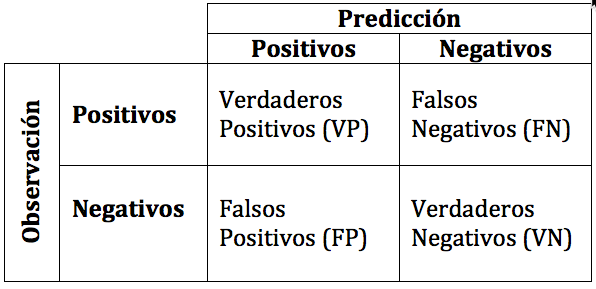
\includegraphics[scale=0.3]{confusionMatrix.png}
			\caption{Representación de la matriz de confusión. Fuente: \href{https://rpubs.com/chzelada/275494}{Rpubs}}
			\label{fig:confusionMatrix}
		\end{figure}
	
	\end{itemize}

	En algunos casos, la \emph{accuracy} puede ser errónea debido a la paradoja de la exactitud donde puede existir un sesgo debido a una distribución desbalanceada de las clases. Esto hace que pueda ser más inteligente elegir un modelo con menor exactitud pero con mayor poder predictivo.
	Para ver ese poder predictivo por lo tanto, es aconsejable elegir más de una métrica de evaluación. Para ello se contará con F1 Score que es la media armónica entre el \emph{recall} y la precisión, y la matriz de confusión que nos permitirá observar como se comporta un modelo especifico preidiciendo las clases.
	
	
	\section{Configuración}
	Aquí hablo del  diseño de los experimentos
	
	
		\printbibliography
	
\end{document}